\documentclass[10pt,a4paper]{article}

% ---------------------------------------------------------------- packages
\usepackage[a4paper,margin=2.2cm]{geometry}
\usepackage[T1]{fontenc}
\usepackage[utf8]{inputenc}
\usepackage{lmodern}
\usepackage{microtype}
\usepackage{amsmath,amssymb}
\usepackage{graphicx}
\usepackage{booktabs}
\usepackage{tabularx}
\usepackage{multirow}
\usepackage{xcolor}
\usepackage{enumitem}
\usepackage{caption}
\usepackage{subcaption}
\usepackage{float}
\usepackage{siunitx}
\usepackage[hidelinks]{hyperref}
\usepackage[capitalise,noabbrev]{cleveref}
\usepackage{listings}
\usepackage{fancyhdr}
\usepackage{parskip}

\graphicspath{{../plots/}}
\sisetup{detect-all}
\setlist{nosep,leftmargin=1.4em}
\captionsetup{font=small,labelfont=bf}
\lstset{basicstyle=\ttfamily\footnotesize,columns=fullflexible,frame=single,framerule=0.3pt,
        backgroundcolor=\color{black!3},xleftmargin=4pt,xrightmargin=4pt}

\pagestyle{fancy}
\fancyhf{}
\lhead{\small CARDIO-CODE}
\rhead{\small DSP arrhythmia detection in motion-corrupted biosignals}
\cfoot{\small\thepage}
\renewcommand{\headrulewidth}{0.3pt}

\newcommand{\code}[1]{\texttt{#1}}
\newcommand{\ibi}{\mathrm{IBI}}

\title{\textbf{CARDIO-CODE}\\[2pt]
\large DSP-Driven Arrhythmia Detection in Motion-Corrupted Biosignals\\[2pt]
\normalsize Technical Report}
\author{Darshan \qquad Piyush\\[4pt]\normalsize Team Ramanujan}
\date{October 2026}

\begin{document}
\maketitle
\thispagestyle{fancy}

\begin{abstract}\setlength{\parindent}{0pt}\setlength{\parskip}{4pt}
\noindent
We present a fully explainable signal-processing pipeline. It converts a noisy wearable biosignal (ECG or PPG) into
four outputs: systolic or R-peak locations, inter-beat intervals (IBIs), a per-sample cardiac-anomaly flag and a
per-sample signal-quality score. No machine learning is used.

\textbf{Baseline wander} is removed by zero-phase Butterworth filtering.

\textbf{In-band motion artifact} in PPG is suppressed in the short-time spectral domain. A harmonic-sum spectrum feeds a
Viterbi heart-rate tracker. Strong non-cardiac spectral lines are re-synthesised and subtracted.

\textbf{Beats} come from two complementary detectors, fused window by window under a noise gate:
\begin{itemize}
  \item a threshold detector (Pan--Tompkins for ECG, Elgendi for PPG);
  \item an HR-guided dynamic-programming (DP) beat selector.
\end{itemize}
The noise gate protects genuinely irregular rhythms such as atrial fibrillation (AF).

\textbf{Anomalies} come from five interpretable rules: pause, bradycardia, premature beat, ectopic morphology and AF-type
irregularity. Every flagged episode can be exported with the rule that fired.

\textbf{Design by measurement.} We developed two complete design branches in parallel and benchmarked them
head to head with one scorer. The final pipeline keeps, component by component, whichever variant measured better.
It combines the detector stack of branch A with these elements of branch B:
\begin{itemize}
  \item robust input handling (time units, jitter, gaps);
  \item accelerometer NLMS motion cancellation;
  \item a mandatory nRMSSD and Poincar\'e test in the AF rule;
  \item a stricter amplitude term in the confidence score.
\end{itemize}

\textbf{Results.}
\begin{itemize}
  \item Supplied record (MIT-BIH 231, intermittent 2:1 AV block): beat $F_1=1.000$, IBI mean absolute error
        \SI{0.99}{ms}, sample-level anomaly $F_1=0.992$.
  \item 44 stress sets (real NSTDB noise, seven real AF/VT records, synthetic motion-corrupted PPG): mean beat
        $F_1=0.925$, mean anomaly $F_1=0.878$. The two design branches alone scored 0.925 / 0.860 and 0.892 / 0.774.
  \item Independent PPG fixture with accelerometer, jittered timestamps and gaps: beat $F_1=0.996$, anomaly $F_1=0.865$.
  \item Runtime: about \SI{2}{s} per \SI{30}{min} record, end to end.
\end{itemize}
\end{abstract}

% =====================================================================================
\section{Problem and data}

\textbf{Task.} Build the layer between a raw wearable signal and an actionable insight. The pipeline outputs
\code{predictions.csv} with one row per sample and five columns:
\code{Timestamp}, \code{Is\_peak}, \code{Ibi\_ms}, \code{ano\_flag} and \code{confidence\_score}.

\textbf{Constraints.} Only time-domain or short-time spectral signal processing is allowed. No ML, NN or pretrained model.

\textbf{Supplied data.} \code{ecg.csv} holds 650\,000 samples at \SI{360}{Hz} (\SI{30.1}{min}) in two leads (MLII, V1).
The file uses the MIT-BIH Arrhythmia Database format. The annotations in \code{annotation.txt} identify the recording as
MIT-BIH record 231: right bundle branch block (RBBB) with intermittent 2:1 second-degree AV block
(\cref{tab:data}).

\begin{table}[h]
\centering\small
\caption{Content of the supplied record, computed from \code{annotation.txt}.}
\label{tab:data}
\begin{tabular}{lrl}
\toprule
Item & Count & Note\\
\midrule
RBBB beats (\code{R}) & 1254 & wide QRS; rSR$'$ in V1\\
Normal beats (\code{N}) & 314 & \\
PVC / APB (\code{V}, \code{A}) & 2 / 1 & all near $t\approx\SI{147}{s}$\\
Dropped beats (\code{MISSB}) & 427 & 420 inside block episodes\\
Rhythm changes \code{(N} $\leftrightarrow$ \code{(BII} & 11 & \\
\midrule
Normal rhythm IBI & -- & $961\pm78$ ms (62 bpm)\\
2:1 block IBI & -- & $1657\pm96$ ms (36 bpm)\\
\bottomrule
\end{tabular}
\end{table}

Two consequences drive the design.
\begin{enumerate}
  \item \textbf{The anomaly is not AF.} A 2:1 block is slow and regular. Classical AF irregularity statistics would miss it.
        The anomaly layer therefore combines several independent rules (\cref{sec:anomaly}).
  \item \textbf{The hidden test set is motion-corrupted PPG with an ECG reference.} The dev data are clean ECG.
        So we built ground-truth stress tests (\cref{sec:eval}) and made the pipeline select ECG or PPG processing
        automatically.
\end{enumerate}

% =====================================================================================
\section{Pipeline overview}

\begin{lstlisting}
CSV -> delimiter sniff, column roles, time-unit detection -> uniform resampling if jittered / gappy
    -> validity mask (NaN runs, time gaps > 1 s) -> ECG-vs-PPG mode -> sanitise (clipping, flat line)
    -> baseline-wander removal -> band limiting -> [ECG] adaptive 50/60 Hz notch
    -> [PPG + ACC] coherence-gated NLMS cancellation, else spectral motion suppression
    -> beat enhancement -> threshold detector + HR-guided DP -> noise-gated fusion
    -> peak refinement (polarity, parabolic sub-sample) -> IBI
    -> beat quality (template correlation x amplitude consistency) -> confidence_score
    -> anomaly rules (pause, bradycardia, premature, morphology, AF) -> ano_flag
\end{lstlisting}

\paragraph{Input handling.}
This layer comes from design branch B.
\begin{itemize}
  \item The delimiter is sniffed from the header. Column roles (time, sample index, PPG, ECG, accelerometer) are
        assigned by name patterns.
  \item The time unit is the one giving a plausible sampling rate (8\,Hz--5\,kHz): s, ms, \si{\micro s} or ns.
        \code{m:ss.sss} and datetime strings are also accepted. Without a time column, \code{--fs} or \SI{360}{Hz} is used.
  \item \textbf{Resampling.} If more than 1\,\% of the intervals deviate from the median by more than 5\,\%, or any
        gap, duplicate or out-of-order stamp exists, the signal is linearly resampled to a uniform grid.
  \item \textbf{Validity.} NaN runs and time gaps longer than \SI{1}{s} are marked invalid. No beats are placed there,
        confidence is 0 and no anomaly is flagged.
  \item \textbf{Output rows.} Results are mapped back to every input row, so the output has exactly one row per input
        sample.
\end{itemize}

\paragraph{Mode detection.}
Without a name hint, the ratio $\rho = P_{10\text{--}40\,\mathrm{Hz}} / P_{0.5\text{--}5\,\mathrm{Hz}}$ of Welch power
decides. $\rho > 0.05$ selects ECG. QRS complexes carry energy above \SI{10}{Hz}; PPG does not. Mode detection is
correct on all 44 test sets.

% =====================================================================================
\section{Baseline wander and motion artifact removal}

\subsection{Baseline wander}
\begin{itemize}
  \item \textbf{ECG.} Second-order zero-phase Butterworth high-pass at \SI{0.5}{Hz} (\code{sosfiltfilt}). This is the
        AHA monitoring cut-off. It removes respiration and electrode or sweat drift without phase distortion of the QRS.
        Detection itself runs in the 5--15\,Hz QRS band, which is insensitive to drift. NSTDB baseline-wander noise at
        \SI{0}{dB} SNR leaves beat $F_1 = 1.000$.
  \item \textbf{PPG.} Zero-phase band-pass 0.5--8\,Hz, the MSPTDfast band~\cite{msptdfast}. It removes the slow
        perspiration-induced coupling drift described in the problem statement. Synthetic drift sets score
        $F_1=1.000$.
\end{itemize}

\subsection{Motion artifact in PPG with an accelerometer: NLMS}
When accelerometer columns are present, a regularised NLMS filter runs at about \SI{25}{Hz}:
\begin{itemize}
  \item 8 taps per axis and step $\mu=0.01$;
  \item the update is $\mathbf w \leftarrow \mathbf w + \mu e\,\mathbf x/(\delta+\|\mathbf x\|^2)$, with
        $\delta=\overline{\|\mathbf x\|^2}$;
  \item the regulariser keeps the step small when the wrist is still;
  \item the filter is applied only if the PPG/ACC coherence in 0.5--5\,Hz exceeds 0.1.
\end{itemize}
The motion estimate is interpolated back to $f_s$ and subtracted. On the accelerometer fixture (motion SNR \SI{0}{dB}), beat
$F_1$ rose from 0.943 to 0.992. Running the spectral line removal of \cref{sec:ms} after NLMS lowered it again. NLMS
alone reached 0.996 (seen in both design branches), so after NLMS the spectral stage only tracks HR.

\subsection{Motion artifact in PPG without an accelerometer: short-time spectral suppression}\label{sec:ms}
Rhythmic arm motion lies inside the cardiac band, so no fixed filter can remove it. Following
TROIKA~\cite{troika}, JOSS~\cite{joss} and harmonic-sum tracking~\cite{hss}, we work in the short-time spectral domain.

\paragraph{1. Spectrum.}
\begin{itemize}
  \item Decimate the band-passed PPG to $f_d\approx\SI{25}{Hz}$. This is at least three times the \SI{8}{Hz} band edge
        and makes the stage 15$\times$ cheaper at \SI{360}{Hz}.
  \item Compute an STFT $X(f,k)$ with an \SI{8}{s} Hann window and a \SI{1}{s} hop.
\end{itemize}

\paragraph{2. Harmonic sum.}
The harmonic sum makes the fundamental win over its own harmonics:
\begin{equation}
  H(f,k) = |X(f,k)| + \tfrac12|X(2f,k)| + \tfrac13|X(3f,k)|, \qquad f\in[0.5, 3.5]\,\mathrm{Hz}.
\end{equation}

\paragraph{3. Viterbi tracking.}
The heart-rate track $f_0(k)$ maximises
\begin{equation}
  \sum_k \log\big(\bar H(f_k,k)+10^{-3}\big) \;-\; \sum_k c(f_{k-1},f_k),
\end{equation}
where $\bar H$ is $H$ normalised per frame and
\begin{equation}
  c(f',f) = \min\big(\lambda|f-f'|,\; J,\; C_{\mathrm{oct}}\,[\,f/f'\approx 2 \text{ or } \tfrac12\,]\big).
  \label{eq:viterbi}
\end{equation}
The cost terms are:
\begin{itemize}
  \item $\lambda=100$ per Hz keeps the track smooth;
  \item the cap $J=10$ allows an abrupt genuine rhythm change, such as the end of a block episode;
  \item $C_{\mathrm{oct}}=4$ makes HR halving or doubling (2:1 block onset) cheap.
\end{itemize}
On the heavy-motion set, frames with $|f_0-\mathrm{HR}_{\mathrm{true}}|>\SI{0.15}{Hz}$ fell from 45\,\% ($\lambda=6$)
to 3--5\,\%.

\paragraph{4. Line removal.}
A bin is a motion line if all three conditions hold:
\begin{itemize}
  \item it is a local spectral maximum;
  \item $|X| > 0.5\,|X(f_0)|$;
  \item it lies more than \SI{0.15}{Hz} from every cardiac harmonic $hf_0$, $h=1..5$.
\end{itemize}
Masked bins (widened to the Hann main lobe) are re-synthesised by inverse STFT, interpolated back to $f_s$ and
subtracted. With an accelerometer, a line must also appear in the accelerometer spectrum.

\paragraph{5. Spectral purity.}
Purity is the share of in-band power within \SI{\pm0.15}{Hz} of the cardiac harmonics. Clean PPG has a 10th percentile
of 0.81; motion bursts have a median of 0.5--0.6. \Cref{fig:ppg} shows the tracker and the suppression.

\subsection{Noise in ECG}
Electrode-motion (EM) and muscle (MA) noise overlap the QRS band. Robustness comes from the detector design
(\cref{sec:dp,sec:fusion}), not from extra filtering. An adaptive 50/60\,Hz notch is applied only if the mains peak
stands more than \SI{10}{dB} above its 2--5\,Hz neighbourhood, so clean files are not touched.

% =====================================================================================
\section{Isolating systolic / R peaks and IBIs under noise}

\subsection{Threshold detectors}
\paragraph{ECG: Pan--Tompkins~\cite{pantompkins}.}
\begin{itemize}
  \item The enhancement signal is $e[n] = \frac1W\sum_{i=0}^{W-1} \big(\dot y[n-i]\big)^2$. Here $y$ is the
        5--15\,Hz band-passed ECG, $\dot y$ its derivative, and $W$ spans \SI{150}{ms}.
  \item Adaptive signal and noise levels give the threshold
        $\theta = \mathrm{NPKI}+0.25(\mathrm{SPKI}-\mathrm{NPKI})$.
  \item The refractory period is \SI{250}{ms}.
  \item Search-back recovers missed beats. When the gap exceeds $1.66\times$ the median RR, the best rejected candidate
        above $\theta/2$ is accepted.
\end{itemize}

\paragraph{PPG: Elgendi~\cite{elgendi2013}.}
\begin{itemize}
  \item Two moving averages (\SI{111}{ms}, \SI{667}{ms}) of the squared positive band-passed PPG define blocks of
        interest.
  \item The offset is $\beta=0.02$ times the local \SI{10}{s} mean, not the global mean. So a motion burst does not
        raise the threshold everywhere.
  \item Blocks shorter than $W_1$ are rejected. The refractory period is \SI{300}{ms}; the larger peak survives.
\end{itemize}

\subsection{HR-guided dynamic-programming beat selection}\label{sec:dp}
\paragraph{Candidates.}
Candidates $i$ are local maxima of the cleaned signal; for ECG, of $\sqrt e$. Each candidate $i$ has a score
$s_i$: the rise amplitude normalised by a rolling 75th percentile and clipped to $[0,1.5]$. Candidates with
$s_i<0.3$ (dicrotic notch, noise) are discarded.

\paragraph{Objective.}
The beat sequence $\mathcal{B}$ maximises
\begin{equation}
  J(\mathcal{B}) = \sum_{i\in\mathcal{B}} s_i \;-\; w\sum_{(j,i)} \min\Big(\Big|\log\tfrac{t_i-t_j}{E(t_i)}\Big|,\;
  \delta + \Big|\log\tfrac{t_i-t_j}{2E(t_i)}\Big|\Big).
  \label{eq:dp}
\end{equation}
The terms are:
\begin{itemize}
  \item $E(t)=1/f_0(t)$, the expected IBI from the spectral track;
  \item $\delta=0.3$, which lets a dropped beat (IBI $\approx 2E$) survive at a small extra cost;
  \item the sum over consecutive chosen beats $(j,i)$ with $t_i-t_j\le\SI{3}{s}$.
\end{itemize}
\Cref{eq:dp} is solved exactly by a Viterbi-style recursion over candidates. A chain restarted after a longer gap
inherits the best earlier chain.

\paragraph{Weight.}
A sweep set $w=3$. Synthetic motion-0.5 $F_1$ was 0.85 at $w=1$ and 0.91 at $w=2.5$--4.

\subsection{Noise-gated fusion}\label{sec:fusion}
The DP prior assumes IBIs follow the tracked HR. That is false in AF: with DP alone, clean-AF PPG sensitivity fell to
0.63. The two detectors are therefore fused in \SI{10}{s} windows.

\paragraph{Rule 1: agreement.}
If at least 90\,\% of beats match within \SI{100}{ms}, keep the threshold detector.

\paragraph{Rule 2: noise gate.}
Let $r$ be the 95th percentile of the enhancement signal \emph{between} beats ($\pm\SI{150}{ms}$ excluded), divided by
its median \emph{at} beats. If $r<g$, the window is clean, however irregular the rhythm, and the threshold detector is
kept. Measured values of $r$ are in \cref{tab:gate}. We use $g=0.45$ for ECG and $g=0.20$ for PPG.

\paragraph{Rule 3: steadiness.}
Otherwise keep the sequence with the smaller median $|\Delta\ibi|$. False detections inflate this statistic; a single
missed beat does not. The comparison is biased towards the threshold detector by a factor of 1.25 (ECG) or 2.2 (PPG).

\begin{table}[h]
\centering\small
\caption{Noise-gate ratio $r$ (median, per \SI{10}{s} window) on representative sets.}
\label{tab:gate}
\begin{tabular}{lc@{\qquad}lc}
\toprule
ECG set & $r$ & PPG set & $r$\\
\midrule
clean (231) & 0.13 & clean synthetic & 0.07\\
real AF (201, 203, 221) & 0.12--0.28 & AF (203, 221) & 0.10--0.18\\
EM 6 dB & 0.39 & motion 0.5 & 0.27--0.29\\
MA 0 dB & 0.41 & & \\
\bottomrule
\end{tabular}
\end{table}

\subsection{Refinement and IBI}
\begin{itemize}
  \item \textbf{ECG polarity.} The R peak is the extremum of the dominant polarity in the 0.5--40\,Hz signal within
        \SI{\pm100}{ms}. This handles inverted leads and the RBBB rSR$'$ shape.
  \item \textbf{Sub-sample timing.} Parabolic interpolation through the three samples around each peak gives
        sub-sample times $t_k$.
  \item \textbf{IBI.} $\ibi_k=t_k-t_{k-1}$. \code{Ibi\_ms} holds the latest IBI until the next beat; it is 0 before the
        second beat.
  \item \textbf{Gate.} IBIs outside \SIrange{0.25}{3}{s} are excluded from the rules.
\end{itemize}

% =====================================================================================
\section{Signal quality: \texorpdfstring{\code{confidence\_score}}{confidence score}}
Following Orphanidou~\cite{orphanidou} and Elgendi~\cite{elgendi2016}, the quality of beat $k$ is
\begin{equation}
  q_k = \max(0,\rho_k)\cdot \exp\!\Big(-\tfrac12\big(\log_2(A_k/\bar A_k)/\sigma\big)^2\Big)\cdot(1-m_k).
\end{equation}
\begin{itemize}
  \item $\rho_k$ is the Pearson correlation of the beat with the median template of all beats within \SI{\pm5}{s}.
  \item $A_k/\bar A_k$ is the beat amplitude relative to the local median amplitude.
  \item $m_k$ is the fraction of clipped, flat-line or invalid samples in the beat window.
\end{itemize}

\paragraph{Two values of $\sigma$.}
The amplitude tolerance $\sigma$ serves two purposes, so it takes two values.
\begin{itemize}
  \item \textbf{Anomaly gate: $\sigma=2$ octaves.} In AF, pulse amplitude legitimately follows the preceding IBI.
        With $\sigma=1$, AF beats looked like noise and anomaly $F_1$ dropped by 0.02.
  \item \textbf{\code{confidence\_score}: $\sigma=0.5$.} This is the stricter amplitude-stability SQI of branch B.
\end{itemize}

\paragraph{Calibration.}
We measured how well the confidence predicts correctness over 4140 \SI{10}{s} windows of the noisy and motion sets.
The measures are the Spearman correlation between window-mean confidence and window beat $F_1$, and the AUC for
predicting $F_1\ge0.9$.
\begin{itemize}
  \item $\sigma=2$: AUC 0.897; $\sigma=0.5$: AUC 0.919, Spearman 0.770. Branch B alone scores 0.919 / 0.785.
  \item Adding branch B's spectral-purity, shape and motion-energy SQIs did not help (AUC 0.843--0.920), so they
        are not used.
\end{itemize}
The per-beat score is interpolated to samples and smoothed with a \SI{2}{s} moving average. It is forced to 0 in
detection gaps longer than \SI{3}{s}, on clipped samples and in invalid regions.

% =====================================================================================
\section{Anomaly detection: \texorpdfstring{\code{ano\_flag}}{anomaly flag}}\label{sec:anomaly}
Each rule uses a reference IBI $R_k$: the median of the previous 8 valid IBIs. A rule is evaluated only when both
beats have $q\ge0.5$ (\cref{tab:rules}).

\begin{table}[h]
\centering\small
\caption{Anomaly rules.}
\label{tab:rules}
\begin{tabularx}{\linewidth}{@{}lXl@{}}
\toprule
Rule & Condition & Targets\\
\midrule
Pause / dropped beat & $\ibi_k > 1.5R_k$ or $\ibi_k>\SI{2}{s}$ & AV block, sinus pause\\
Bradycardia & 5-beat median HR $<45$ bpm & 2:1 AV block, severe bradycardia\\
Premature beat & $\ibi_k<0.8R_k$ and $\ibi_k+\ibi_{k+1}>1.6R_k$ (compensatory pause) & PVC, APB\\
Ectopic morphology (ECG) & $\rho_k<0.8$, neighbours $>0.9$, $\ibi_k<0.92R_k$ & PVC\\
AF irregularity & 16-beat window: $\mathrm{med}|\Delta\ibi|/\mathrm{med}\,\ibi>0.10$ and
                  $\mathrm{RMSSD}/\overline{\ibi}>0.15$ and (turning-point count within $\pm2\sigma$ of a random
                  series~\cite{dash} or Poincar\'e $\mathrm{SD1}/\mathrm{SD2}>0.6$) & AF, flutter\\
\bottomrule
\end{tabularx}
\end{table}

\paragraph{Why a median statistic for AF.}
The median of $|\Delta\ibi|$ is robust to isolated ectopic beats. An earlier version excluded IBIs next to premature
beats instead. In real AF most windows then fell below the coverage limit and were skipped.

\paragraph{Threshold choice.}
We swept the median-statistic threshold on seven MIT-BIH AF records (\cref{fig:af}). Mean anomaly $F_1$ was 0.908 at
0.08, 0.915 at 0.10, 0.907 at 0.12 and 0.884 at 0.15.

\paragraph{Additions from branch B.}
\begin{itemize}
  \item \textbf{Mandatory nRMSSD.} Over 46 sets, anomaly $F_1$ was 0.8661 without it, 0.8720 at 0.12, 0.8742 at 0.15
        and 0.8712 at 0.18. At 0.15 it removes a \SI{19.5}{s} false AF episode caused by respiratory sinus arrhythmia
        in \code{ecg.csv}.
  \item \textbf{Poincar\'e SD1/SD2} as an alternative to the turning-point test: 0.8654 with TPR only, 0.8661 with
        either test.
\end{itemize}

\paragraph{From beats to samples.}
A flagged beat flags its IBI span; a premature beat also flags the following span. Spans are not dilated. Gaps shorter
than \SI{6}{s} between flagged spans are closed, because AF episodes contain short regular-looking stretches. A
\SI{0.5}{s} dilation (v6) cost precision: \code{ecg.csv} anomaly $F_1$ was 0.974, versus 0.982 without it.

\paragraph{Explainable output.}
\code{--events} writes every episode with its rule, a plain-text reason, start and end time, number of beats and median
IBI. \code{--annotation} prints beat Se/PPV/$F_1$, IBI MAE and anomaly Se/PPV/$F_1$. For PPG, the PPG-to-ECG lag is
estimated and removed before matching.

% =====================================================================================
\section{Evaluation}\label{sec:eval}
\subsection{Stress-test data}
\begin{itemize}
  \item \textbf{ECG with real noise.} Record 231 plus NSTDB~\cite{nstdb} electrode-motion (em), muscle (ma) and
        baseline-wander (bw) noise. Levels are 12, 6 and \SI{0}{dB} SNR, with $S=\mathrm{pp}_{\mathrm{QRS}}^2/8$ (the
        \code{nst} definition). One extra set mixes all three in \SI{2}{min} bursts.
  \item \textbf{Real arrhythmias.} MIT-BIH records 201, 202, 203, 210, 219, 221 and 222, which contain AF, flutter,
        VT, bigeminy, SVTA and nodal rhythm. They are read with our own WFDB annotation parser.
  \item \textbf{Synthetic PPG} at 64, 125 and \SI{360}{Hz}, driven by the annotated beat times:
        \begin{itemize}
          \item two-Gaussian pulse at R $+$ PTT ($\approx\SI{220}{ms}$);
          \item Frank--Starling amplitude scaling;
          \item weak pulses for ectopic beats;
          \item respiration;
          \item variants with drift and in-band harmonic motion (0.8--1.6\,Hz sweep in \SI{30}{s} bursts, plus jolts).
        \end{itemize}
\end{itemize}

\subsection{Metrics}
\begin{itemize}
  \item Beats are matched within \SI{\pm150}{ms} (AAMI EC57); we report sensitivity (Se), positive predictive value
        (PPV) and $F_1$.
  \item IBI mean absolute error (MAE) is computed over consecutive matched pairs.
  \item Anomaly $F_1$ is per sample. The ground truth is non-sinus rhythm segments, spans around ectopic beats, and
        dropped-beat pauses.
  \item Window $F_1$ uses \SI{10}{s} windows.
  \item Runtime is measured for \SI{30}{min} of signal on one CPU core.
\end{itemize}

\subsection{Results}
\Cref{tab:results} lists the results; \cref{fig:bench} compares the first version with the final pipeline.

\begin{table}[h]
\centering\small
\caption{Results of the final pipeline. Ranges cover the seven MIT-BIH arrhythmia records or the three PPG
sampling rates. Time: processing of the record (stress sets) or the full command including CSV input/output (fixtures).}
\label{tab:results}
\resizebox{\linewidth}{!}{%
\begin{tabular}{lccccc}
\toprule
Dataset & beat $F_1$ & IBI MAE (ms) & anomaly $F_1$ & window $F_1$ & time (s)\\
\midrule
\textbf{ecg.csv (record 231)} & \textbf{1.000} & \textbf{1.0} & \textbf{0.992} & 0.994 & $\le$0.46\\
\quad + baseline wander 12 / 6 / \SI{0}{dB} & 1.000 & 1.0 & 0.984--0.992 & 0.988--0.994 & $\le$0.45\\
\quad + muscle artifact 12 / 6 / \SI{0}{dB} & 1.000 / 0.994 / 0.941 & 1.1 / 1.5 / 3.7 & 0.992 / 0.988 / 0.906 & 0.994 / 0.981 / 0.894 & $\le$0.49\\
\quad + electrode motion 12 / 6 / \SI{0}{dB} & 0.999 / 0.924 / 0.776 & 1.0 / 2.5 / 14.5 & 0.991 / 0.872 / 0.484 & 0.994 / 0.894 / 0.593 & $\le$0.52\\
\quad + mixed bursts \SI{6}{dB} & 0.976 & 1.8 & 0.938 & 0.957 & $\le$0.47\\
\midrule
MIT-BIH AF/VT, ECG (7) & 0.971--0.999 & 1.0--15.8 & 0.866--0.997 & 0.938--1.000 & $\le$0.65\\
MIT-BIH AF/VT, PPG clean (7) & 0.927--0.986 & 5.3--8.7 & 0.858--1.000 & 0.918--1.000 & $\le$0.45\\
MIT-BIH AF/VT, PPG + motion (7) & 0.778--0.855 & 14.8--19.9 & 0.592--0.980 & 0.697--0.997 & $\le$0.43\\
\midrule
Synthetic PPG clean / drift (64--360 Hz) & 1.000 & 1.5--5.8 & 0.980--0.990 & 0.981--0.994 & $\le$0.38\\
Synthetic PPG motion 0.5 & 0.844--0.860 & 17.9--19.9 & 0.688--0.773 & 0.693--0.765 & $\le$0.43\\
Synthetic PPG motion 1.0 & 0.722--0.738 & 23.7--26.3 & 0.527--0.552 & 0.578--0.605 & $\le$0.45\\
\midrule
Fixture, PPG + ACC (\SI{0}{dB} motion) & 0.996 & 8.2 & 0.865 & -- & 1.18\\
Fixture, PPG, no ACC & 0.943 & 12.2 & 0.730 & -- & 1.07\\
\bottomrule
\end{tabular}}
\end{table}

\paragraph{Totals.}
Over all 44 stress sets: mean beat $F_1=0.925$, anomaly $F_1=0.878$ and window $F_1=0.910$.
\Cref{sec:merge} compares these with the two design branches.

\paragraph{Runtime.}
The end-to-end command, including parsing and writing 650\,000 CSV rows, takes about \SI{2}{s}.

\begin{figure}[p]
\centering
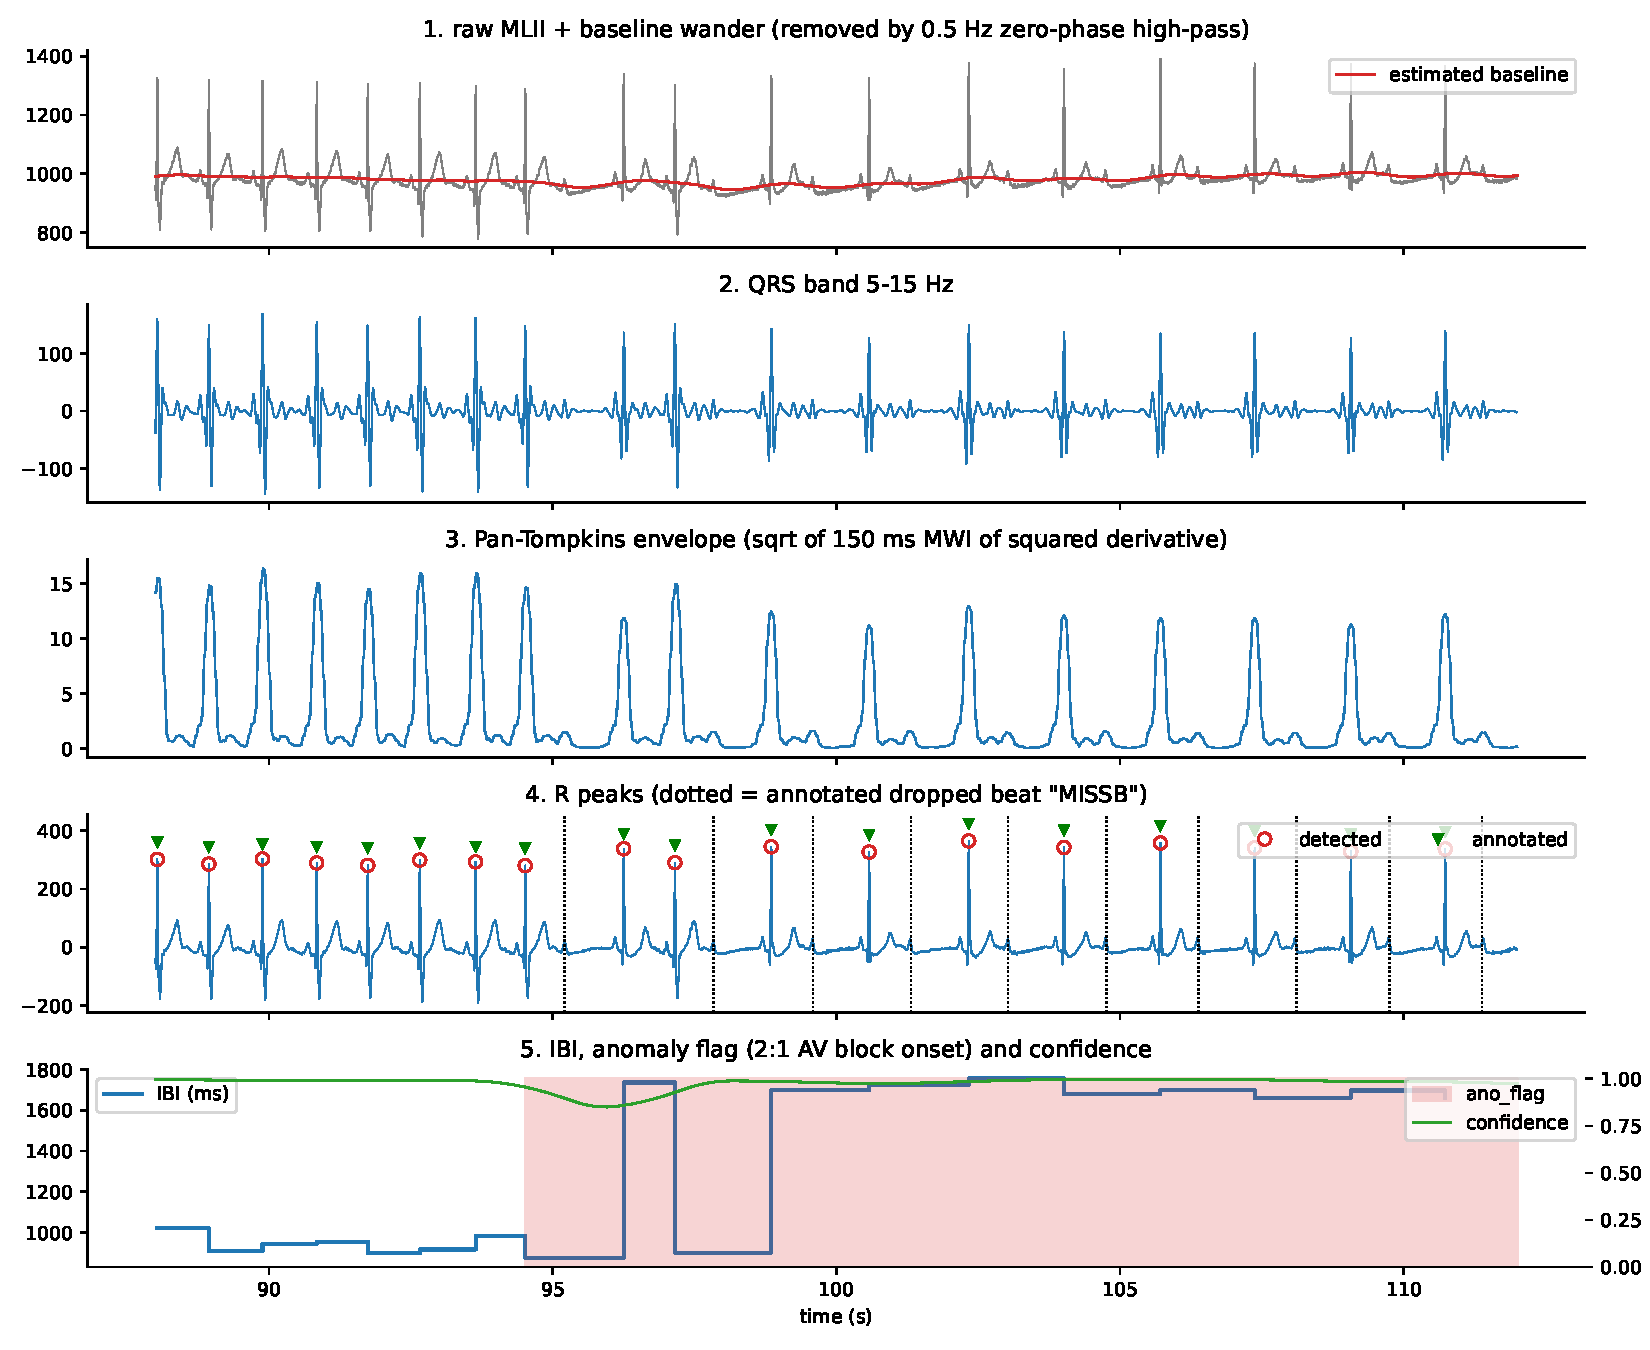
\includegraphics[width=\linewidth]{fig1_ecg_stages.pdf}
\caption{ECG pipeline stages around the onset of 2:1 AV block in \code{ecg.csv}: raw signal with estimated baseline,
QRS band, Pan--Tompkins envelope, detected vs annotated R peaks (dotted lines: dropped beats), and IBI with
\code{ano\_flag} and \code{confidence\_score}.}
\label{fig:ecg}
\end{figure}

\begin{figure}[p]
\centering
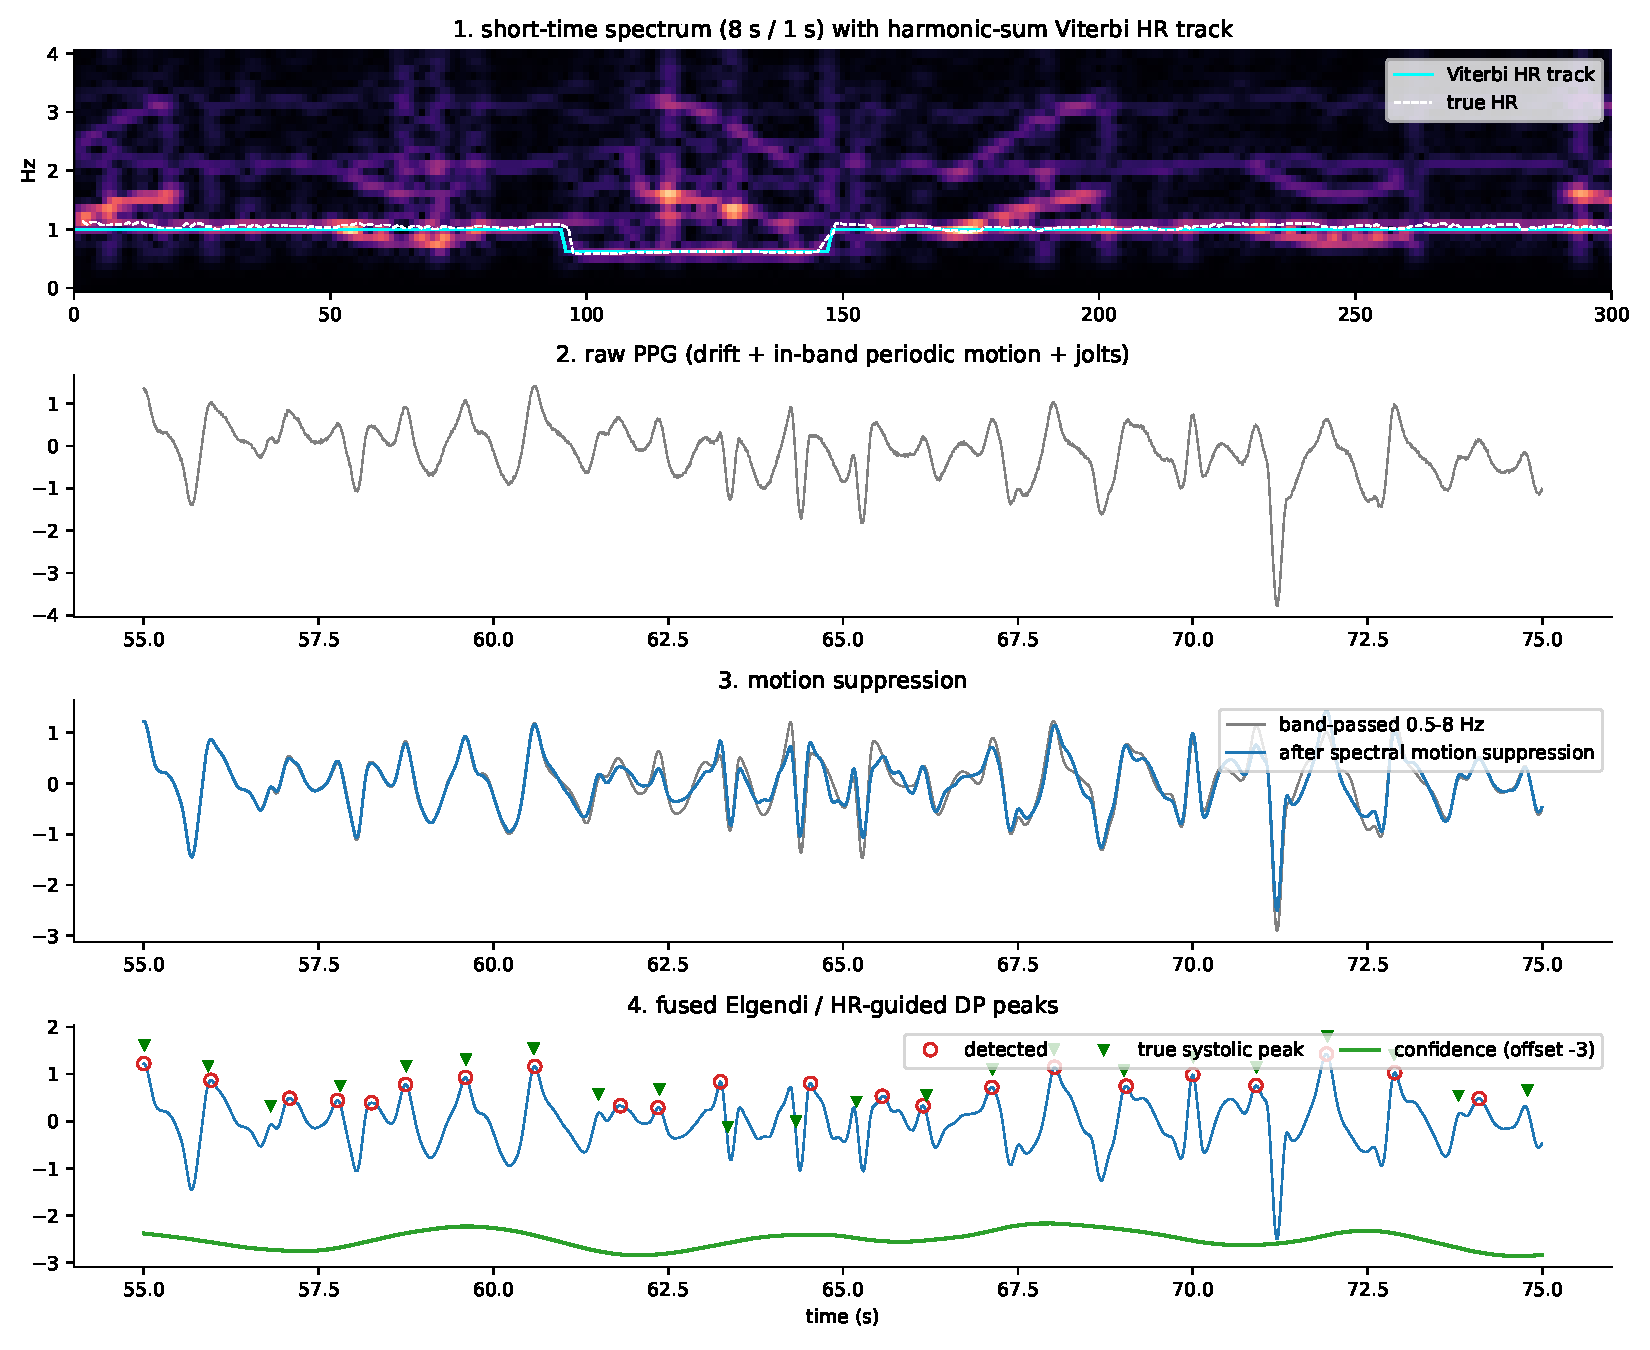
\includegraphics[width=\linewidth]{fig2_ppg_motion.pdf}
\caption{PPG motion handling (synthetic motion level 0.5): STFT with the Viterbi HR track vs true HR, raw PPG, PPG
before and after spectral motion suppression, and fused detections with the confidence score.}
\label{fig:ppg}
\end{figure}

\begin{figure}[t]
\centering
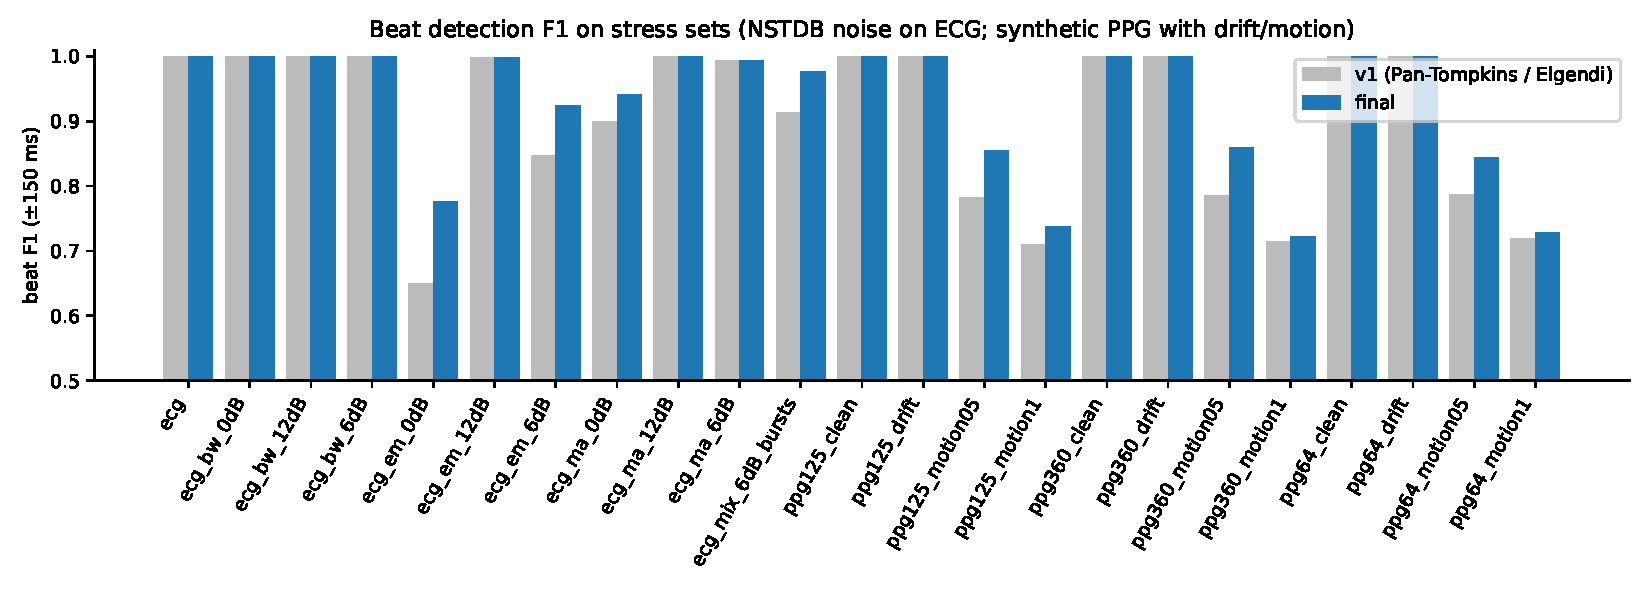
\includegraphics[width=\linewidth]{fig3_benchmark.pdf}
\caption{Beat $F_1$ per stress set: first version (plain Pan--Tompkins / Elgendi) vs final pipeline.}
\label{fig:bench}
\end{figure}

\begin{figure}[t]
\centering
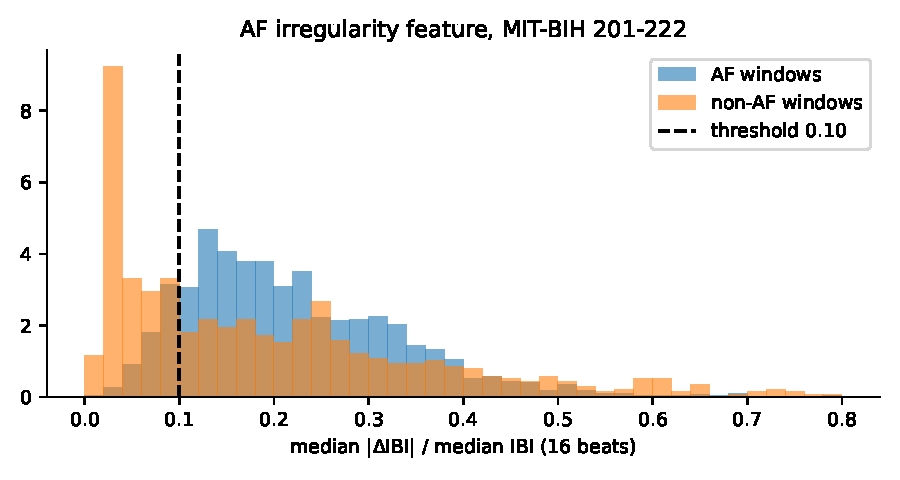
\includegraphics[width=0.62\linewidth]{fig4_af_feature.pdf}
\caption{Distribution of the AF irregularity statistic in 16-beat windows, AF vs non-AF, MIT-BIH records 201--222. The
dashed line marks the chosen threshold.}
\label{fig:af}
\end{figure}

% =====================================================================================
\section{Design branches and component selection}\label{sec:merge}
To avoid locking in early design choices, we developed two complete design branches in parallel:
\begin{itemize}
  \item \textbf{branch A}: noise-gated detector fusion, HR-guided DP and spectral motion suppression;
  \item \textbf{branch B}: robust input layer, NLMS accelerometer cancellation, Pan--Tompkins-style detector, 4-rule
        anomaly logic with a quality gate, and 5-SQI confidence.
\end{itemize}

\paragraph{Protocol.}
Both branches, and the final pipeline, ran as command-line programs on identical files. One scorer read only
their \code{predictions.csv}.
\begin{itemize}
  \item The 44 stress sets were used to tune branch A, so they may favour it.
  \item A second, independently generated set of synthetic PPG fixtures was therefore added: \SI{64}{Hz} with timestamp jitter, NaN runs and a
        dropped block; AF, PVCs and dropped beats; in-band motion at \SI{0}{dB}; with or without a 3-axis accelerometer.
  \item Peaks on the fixtures are matched after removing each branch's own median PPG-to-ECG lag.
  \item The common scorer reproduces branch B's built-in validation on these fixtures (anomaly $F_1$ 0.705 and 0.357).
\end{itemize}

\paragraph{Outcome.}
Branch A was better overall. Branch B was better on:
\begin{itemize}
  \item clean-signal anomaly precision;
  \item PPG with an accelerometer (A ignored ACC columns, a bug);
  \item irregular time axes;
  \item confidence calibration.
\end{itemize}
Each B component was then added to A and kept only if it helped (\cref{tab:merge}, \cref{fig:merge}).

\begin{table}[h]
\centering\small
\caption{Head-to-head means over dataset groups: branch A / branch B / final pipeline. Beat $F_1$ and
sample-level anomaly $F_1$; one scorer, identical inputs.}
\label{tab:merge}
\begin{tabular}{lccc@{\qquad}ccc}
\toprule
 & \multicolumn{3}{c}{beat $F_1$} & \multicolumn{3}{c}{anomaly $F_1$}\\
Group & A & B & final & A & B & final\\
\midrule
ecg.csv & 1.000 & 1.000 & 1.000 & 0.974 & \textbf{0.995} & 0.992\\
ECG + NSTDB noise (10) & \textbf{0.961} & 0.937 & \textbf{0.961} & 0.894 & 0.733 & \textbf{0.914}\\
Real AF/VT ECG (7) & 0.991 & \textbf{0.994} & 0.991 & 0.908 & 0.873 & \textbf{0.920}\\
Real AF/VT PPG, clean (7) & 0.963 & \textbf{0.967} & 0.963 & 0.912 & \textbf{0.928} & \textbf{0.928}\\
Real AF/VT PPG, motion (7) & \textbf{0.811} & 0.742 & \textbf{0.811} & 0.831 & 0.599 & \textbf{0.840}\\
Synthetic PPG, clean / drift (6) & 1.000 & 0.999 & 1.000 & 0.967 & \textbf{0.994} & 0.983\\
Synthetic PPG, motion (6) & \textbf{0.791} & 0.657 & \textbf{0.791} & 0.592 & 0.491 & \textbf{0.628}\\
\midrule
\textbf{All 44 stress sets} & \textbf{0.925} & 0.892 & \textbf{0.925} & 0.860 & 0.774 & \textbf{0.878}\\
Fixture, PPG + ACC & 0.943 & 0.987 & \textbf{0.996} & 0.734 & 0.705 & \textbf{0.865}\\
Fixture, PPG, no ACC & \textbf{0.943} & 0.851 & \textbf{0.943} & \textbf{0.734} & 0.357 & 0.730\\
\bottomrule
\end{tabular}
\end{table}

\begin{figure}[h]
\centering
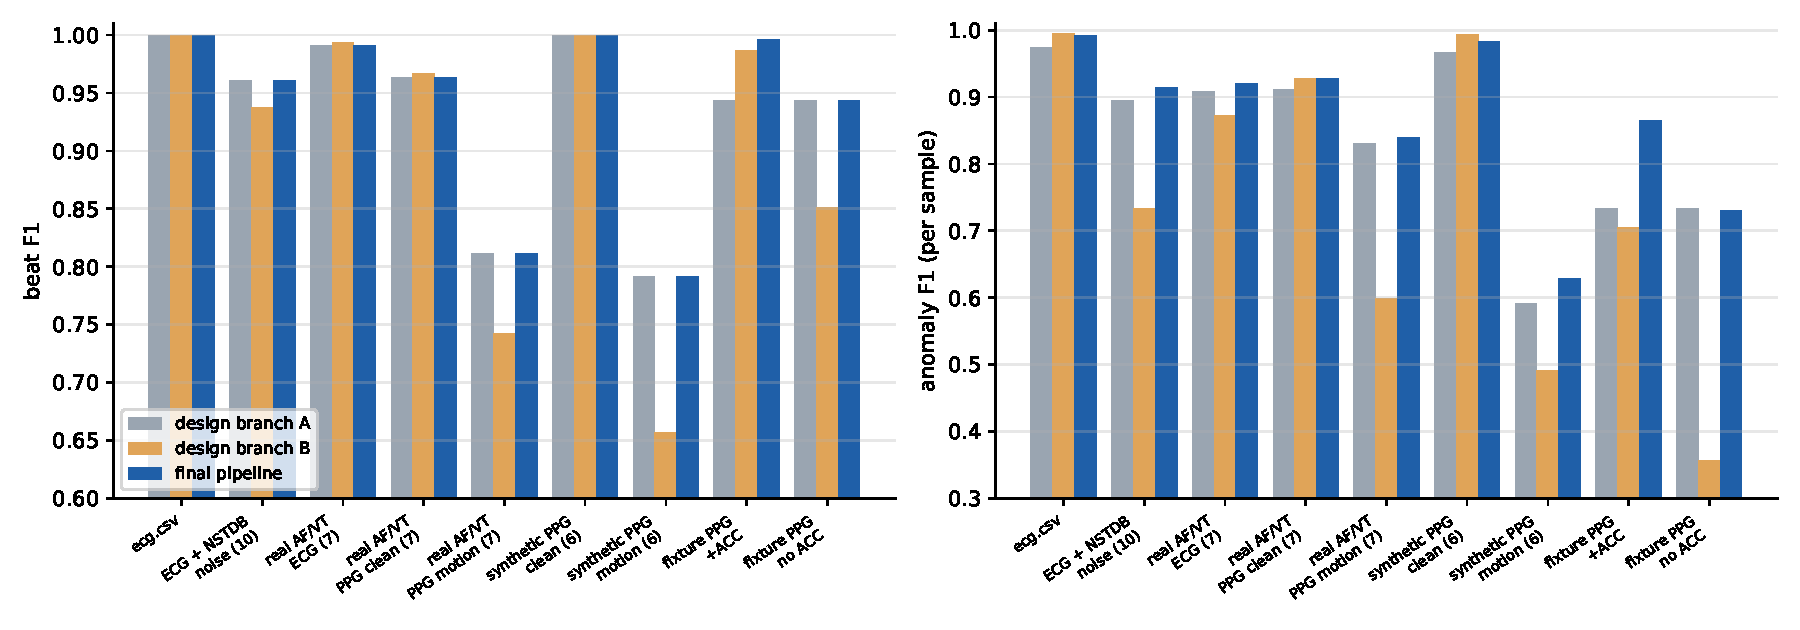
\includegraphics[width=\linewidth]{fig5_compare.pdf}
\caption{Head-to-head: design branch A, design branch B and final pipeline.}
\label{fig:merge}
\end{figure}

\paragraph{Taken from branch B (measured gains).}
\begin{itemize}
  \item input layer and validity mask (\code{ecg.csv} output byte-identical, fixtures handled natively);
  \item coherence-gated NLMS (fixture beat $F_1$ 0.943 $\to$ 0.996);
  \item mandatory nRMSSD and SD1/SD2 in the AF rule (anomaly $F_1$ 0.866 $\to$ 0.874);
  \item no span dilation (\code{ecg.csv} 0.974 $\to$ 0.982 before the AF change);
  \item stricter amplitude term in the confidence (AUC 0.897 $\to$ 0.919);
  \item adaptive mains notch.
\end{itemize}

\paragraph{Not adopted.}
\begin{itemize}
  \item B's 5-SQI confidence fusion (AUC fell to 0.861);
  \item B's 40\,bpm bradycardia threshold (no gain);
  \item B's single Pan--Tompkins-style detector, which is weaker under noise than A's fused detectors
        (beat $F_1$ 0.892 vs 0.925).
\end{itemize}

\paragraph{Where B is still ahead.}
\begin{itemize}
  \item Real AF/VT ECG: beat $F_1$ 0.994 vs 0.991, IBI MAE 3.0 vs \SI{4.4}{ms}. B uses secondary-wave rejection and
        refines peaks on the cleaned signal.
  \item Clean synthetic-PPG anomaly $F_1$: 0.994 vs 0.983.
\end{itemize}
Adding B's detector as a third fusion candidate is the natural next step.

% =====================================================================================
\section{Development history and rejected ideas}
Each change was measured on the full stress suite before adoption (\cref{tab:history}).

\begin{table}[h]
\centering\small
\caption{Development history.}
\label{tab:history}
\begin{tabularx}{\linewidth}{@{}lXX@{}}
\toprule
Version & Change & Effect\\
\midrule
v1 & Pan--Tompkins / Elgendi, rule-based anomalies, template SQI & ecg.csv perfect; PPG + motion $F_1$ 0.71--0.78\\
v2 & Spectral motion suppression, Viterbi HR track, DP beat selection & motion-0.5 $F_1$ 0.78 $\to$ 0.83\\
v3 & Fixed STFT hop-timing bug (track drifted \SI{50}{s} over \SI{30}{min}); DP weight 3; ECG fusion
   & mean beat $F_1$ 0.904 $\to$ 0.941; EM \SI{6}{dB} 0.85 $\to$ 0.94\\
v4 & Real AF/VT records added; noise-gated fusion; AF-rule fix & clean-AF PPG Se 0.63 $\to$ 0.88--0.99\\
v5 & AF-tolerant amplitude term in beat quality & anomaly $F_1$ 0.841 $\to$ 0.860\\
v6 & Template-correlation peak refinement; stricter quality gates & no gain (rejected)\\
v7 & Component selection across branches A and B: input layer, NLMS, AF nRMSSD + SD1/SD2, span merging, strict confidence
   & anomaly $F_1$ 0.860 $\to$ 0.878; ecg.csv 0.974 $\to$ 0.992; fixture + ACC beat $F_1$ 0.943 $\to$ 0.996\\
\bottomrule
\end{tabularx}
\end{table}

These ideas were tested and rejected:
\begin{itemize}
  \item a purity-adaptive HR-prior weight;
  \item switching detectors by a motion indicator;
  \item vetoing a pause when its gap holds an undetected pulse-sized peak ($-0.001$ anomaly $F_1$);
  \item template cross-correlation peak refinement. IBI MAE rose from 19.5 to \SI{21}{ms}: under motion the error comes
        from wrong-crest picks, not jitter.
\end{itemize}

% =====================================================================================
\section{Limitations}
\begin{itemize}
  \item \textbf{Very strong in-band motion.} When motion amplitude exceeds pulse amplitude, beat $F_1$ is about 0.73.
        The confidence score correctly drops there (mean 0.75, vs 0.99 when clean).
  \item \textbf{Anomaly precision in noisy PPG} is lower: missed or extra beats mimic pauses and irregularity.
  \item \textbf{Evaluation bias.} The stress sets were also used for tuning. The second fixture set provides an
        independent check, but the hidden test set may differ in morphology and noise.
  \item \textbf{Synthetic PPG.} The PPG test signals use pulse shapes driven by real beat times. Real PPG morphology
        varies more.
  \item \textbf{PPG peak lag.} A PPG systolic peak lags the ECG R peak by the pulse transit time. We report the
        detected systolic time without shifting it.
\end{itemize}

% =====================================================================================
\begin{thebibliography}{99}\small
\bibitem{pantompkins} J.~Pan, W.~J.~Tompkins, ``A real-time QRS detection algorithm,'' \emph{IEEE Trans. Biomed. Eng.}, 32(3), 1985.
\bibitem{elgendi2013} M.~Elgendi et al., ``Systolic peak detection in acceleration photoplethysmograms measured from emergency responders in tropical conditions,'' \emph{PLoS ONE}, 8(10), 2013.
\bibitem{charlton2022} P.~H.~Charlton et al., ``Detecting beats in the photoplethysmogram: benchmarking open-source algorithms,'' \emph{Physiol. Meas.}, 43, 085007, 2022.
\bibitem{msptdfast} P.~H.~Charlton et al., ``The MSPTDfast photoplethysmography beat detection algorithm: design, benchmarking, and open-source distribution,'' \emph{Physiol. Meas.}, 2025.
\bibitem{troika} Z.~Zhang, Z.~Pi, B.~Liu, ``TROIKA: a general framework for heart rate monitoring using wrist-type photoplethysmographic signals during intensive physical exercise,'' \emph{IEEE Trans. Biomed. Eng.}, 62(2), 2015.
\bibitem{joss} Z.~Zhang, ``Photoplethysmography-based heart rate monitoring in physical activities via joint sparse spectrum reconstruction,'' \emph{IEEE Trans. Biomed. Eng.}, 62(8), 2015.
\bibitem{hss} ``Harmonic sum-based method for heart rate estimation using PPG signals affected with motion artifacts,'' arXiv:1610.05112, 2016.
\bibitem{orphanidou} C.~Orphanidou et al., ``Signal-quality indices for the electrocardiogram and photoplethysmogram,'' \emph{IEEE J. Biomed. Health Inform.}, 19(3), 2015.
\bibitem{elgendi2016} M.~Elgendi, ``Optimal signal quality index for photoplethysmogram signals,'' \emph{Bioengineering}, 3(4), 2016.
\bibitem{dash} S.~Dash et al., ``Automatic real time detection of atrial fibrillation,'' \emph{Ann. Biomed. Eng.}, 37(9), 2009.
\bibitem{bonomi} A.~G.~Bonomi et al., ``Comparison between ECG- and PPG-derived features for atrial fibrillation detection in free-living conditions,'' \emph{Physiol. Meas.}, 39, 2018.
\bibitem{nstdb} G.~B.~Moody, W.~Muldrow, R.~G.~Mark, ``A noise stress test for arrhythmia detectors,'' \emph{Computers in Cardiology}, 1984; MIT-BIH Arrhythmia and Noise Stress Test Databases, PhysioNet.
\end{thebibliography}

\end{document}
